\section{Analisi teorica}


\begin{frame}
  \frametitle{Funzione di partizione}
  \framesubtitle{}
  
  \centering
  Studiamo il sistema nell'ensamble gran canonico $\left(\mu,\,V,\,T\right)$

  $$
    Z\left(T,\,V,\,z\right)\,=\,\prod_i \frac{1}{1\,-\,z\exp{\left(-\beta \varepsilon_i \right)}}
  $$

  \vspace{20pt}
  \centering
  La funzione di partizione consente di ricavare la termodinamica del sistema
  $$
    N\,=\,\frac{z\exp{\left(-\beta \varepsilon_0 \right)}}{1\,-\,z\exp{\left(-\beta \varepsilon_0 \right)}}\,+\,\sum_{i \neq 0}\left<n_i\left(\mu,\,T\right)\right>
  $$
  $$
  \left<\hat{H}\right>\,=\,\sum_i \varepsilon_i \left<n_i\right>
  $$

\end{frame}


\begin{frame}
  \frametitle{Frazione di condensato}
  \framesubtitle{}

  \begin{columns}
      \begin{column}{0.5\textwidth}
        $$
        \frac{N_0}{N}\,=\,
        \begin{cases}
        0 \qquad \qquad \qquad \qquad T \geq T_c \\
        1\,-\,\left(T/T_c\right)^{3/2} \qquad \,T < T_c
        \end{cases}
        $$
        $$
        \frac{N_T}{N}\,=\,
        \begin{cases}
        1 \qquad \qquad \qquad \qquad T \geq T_c \\
        \left(T/T_c\right)^{3/2} \qquad \qquad \,\,T < T_c
        \end{cases}
        $$
      \end{column}
      
      \begin{column}{0.5\textwidth}
        \begin{figure}
            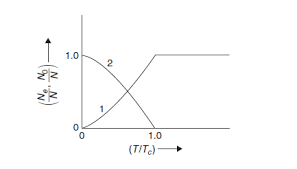
\includegraphics[width=\textwidth]{Immagini/frazCond.png}
            \caption{Frazione di condensato in funzione della temperatura.}
        \end{figure}
      \end{column}
    \end{columns}

\end{frame}


\begin{frame}
  \frametitle{Calore specifico}
  \framesubtitle{}

  \begin{columns}
      \begin{column}{0.5\textwidth}
        $$
        \left<\hat{H}\right>\,=\,\frac{3}{2}k_B T\frac{V}{\lambda_T^3}g_{5/2}\left(z\right)
        $$
        \vspace{12pt}
        \begin{itemize}[itemsep=0.5em, label=$\bullet$]
          \item punto angoloso a $T_c$
          \item recupero il risultato valido per il gas ideale nel limite $T \rightarrow \infty$.
        \end{itemize}
      \end{column}
      
      \begin{column}{0.5\textwidth}
        \begin{figure}
            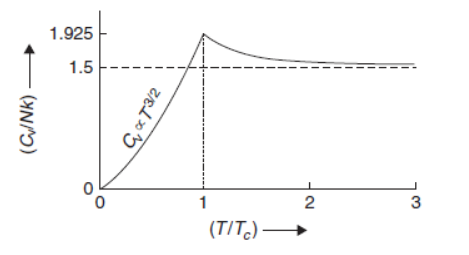
\includegraphics[width=\textwidth]{Immagini/calSpe.png}
            \caption{Calore specifico del gas di Bose ideale}
        \end{figure}
      \end{column}
    \end{columns}

\end{frame}